%----------
%	HATE SPEECH IN SOCIAL MEDIA
%----------	

As we have seen in the previous Section of this Chapter, hate speech is undoubtedly present in society and it is manifested in different ways. Mass media and, in particular, social networks are the perfect vehicle for spreading this type of toxic content.

There are multiple factors that contribute to the proliferation of sexist hate speech, such as the prevalence of patriarchal societies, the expectations about women and men’s sexuality and roles in society, and the dissemination of degrading images and messages about women or girls notably in the media\footnote{From \url{https://www.coe.int/en/web/genderequality/sexist-hate-speech}, last visited 16/08/24}. In Spain, there are a couple of initiatives that have been carried out by different institutions and civil societal organizations (CSOs). 

GeMeCo (Visualización de Brechas de Género en Medios de Comunicación)\footnote{From \url{https://gemeco.ujaen.es/}, last visited 07/08/24} is an online tool developed by the SINAI group (Sistemas Inteligentes de Acceso a la Información) of the Universidad de Jaén, that as shown in Figure~\ref{fig:gemeco}, show the proportion of men and women that are being cited in the most popular and influential media in Spain. This project is the Spanish version of the GenderGap Tracker\footnote{From \url{https://gendergaptracker.informedopinions.org/}, last visited 07/08/24}, that was developed by the Simon Fraser University in Canada, and that performs the same analysis but in the francophone media.

\begin{figure}[H]
	\ffigbox[\FBwidth]
	{\caption{Proportion of Women and Men Cited in the News of the Most Influential Online Media in Spain, from 01/01/2024 to 01/08/2024. Retrieved from \url{https://gemeco.ujaen.es/}}\label{fig:gemeco}} 
 % [Aquí ponemos como queremos que aparezca en el índice, sin la referencia]{Aquí como queremos que aparezca en el documento, con la referencia}
	{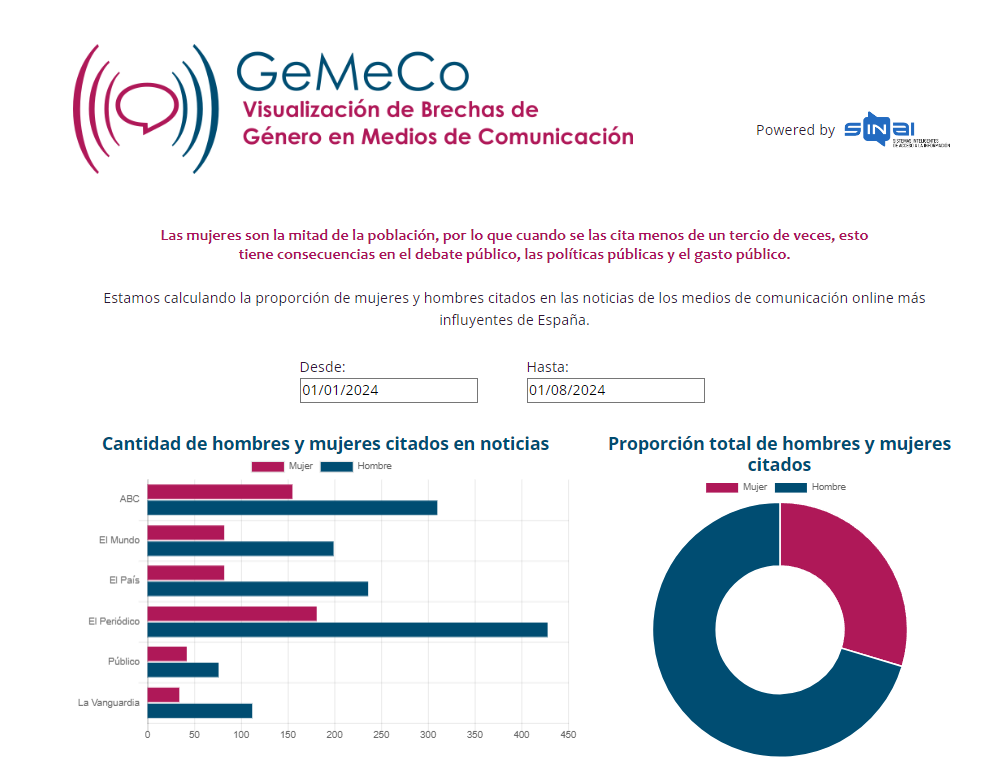
\includegraphics[scale=0.5]{Plantilla_TFG_ingles_2019/imagenes/gemeco.png}}
\end{figure}

Since May 2020 another remarkable project has been developed by the The Spanish Observatory of Racism and Xenophobia (OBERAXE)\footnote{From \url{https://www.inclusion.gob.es/oberaxe/es/ejes/discursoodio/index.htm}, last visited 07/08/24}. It consists of a bimonthly Bulletin about the Monitorization of online hate speech in Spain. For that purpose, daily systematic monitoring of this content is carried out on the most important data hosting service platforms (YouTube, Twitter/X, Facebook, Instagram and TikTok).


HateMedia\footnote{From \url{https://www.hatemedia.es/resultados-hatemedia/}, last visited 07/08/24} is another initiative funded by the Ministry of Science and Innovation, and the Statal Investigation Agency of Spain, which aims to analyze how hate speech spreads in digital environments and to enhance the detection and monitoring of such expressions in Spanish media. In particular, they have developed the "Monitor de Odio" (eng. `Hate Monitor´, Figures~\ref{fig:hatemedia1} and~\ref{fig:hatemedia2}), which was created to provide a general indicator of the presence, intensity, and most common types of hate expressions in Spanish media. It distinguishes hate characteristics based on the presence of hate expressions, the type of hate detected (general, political, sexual, misogynistic, or xenophobic) and the intensity of hate (levels 1 to 4).


\begin{figure}[H]
	\ffigbox[\FBwidth]
	{\caption{Dashboard of the Hatemedia's Monitor of Speech on 16/08/2024. Retrieved from \url{https://monitordeodio.hatemedia.es/#/}}\label{fig:hatemedia1}} 
 % [Aquí ponemos como queremos que aparezca en el índice, sin la referencia]{Aquí como queremos que aparezca en el documento, con la referencia}
	{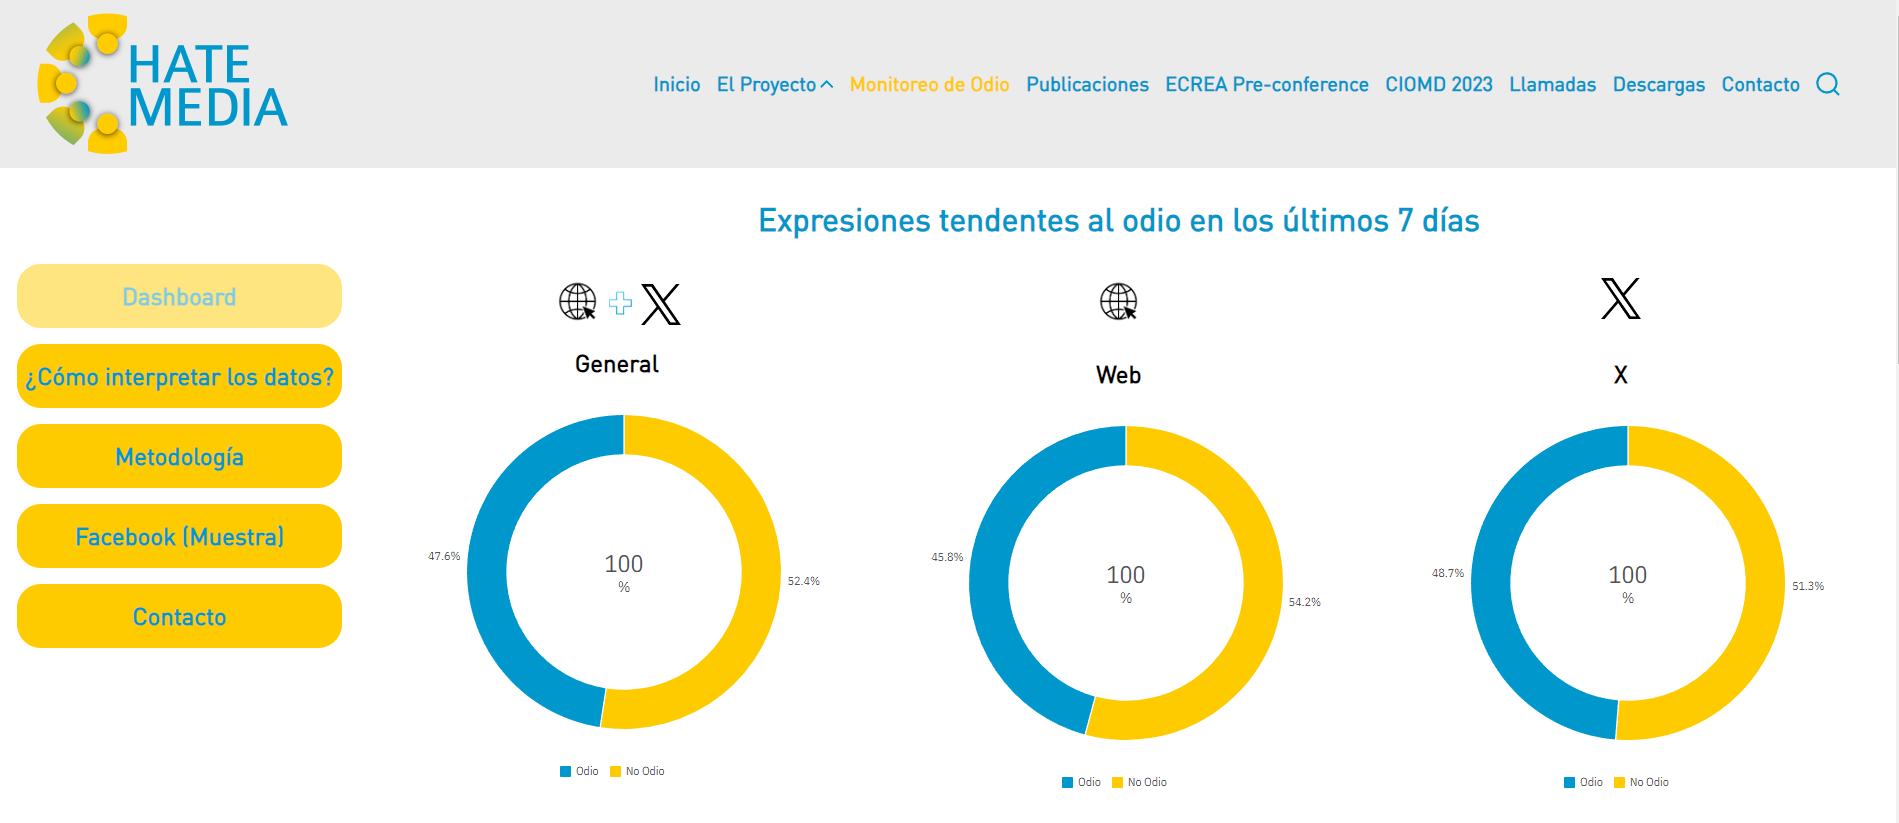
\includegraphics[scale=0.25]{Plantilla_TFG_ingles_2019/imagenes/hatemedia1.png}}
\end{figure}


\begin{figure}[H]
	\ffigbox[\FBwidth]
	{\caption{Proportion of the Different Types of Hate Analysed by Hatemedia's Monitor of Speech on 16/08/2024. Retrieved from \url{https://monitordeodio.hatemedia.es/#/}}\label{fig:hatemedia2}} 
 % [Aquí ponemos como queremos que aparezca en el índice, sin la referencia]{Aquí como queremos que aparezca en el documento, con la referencia}
	{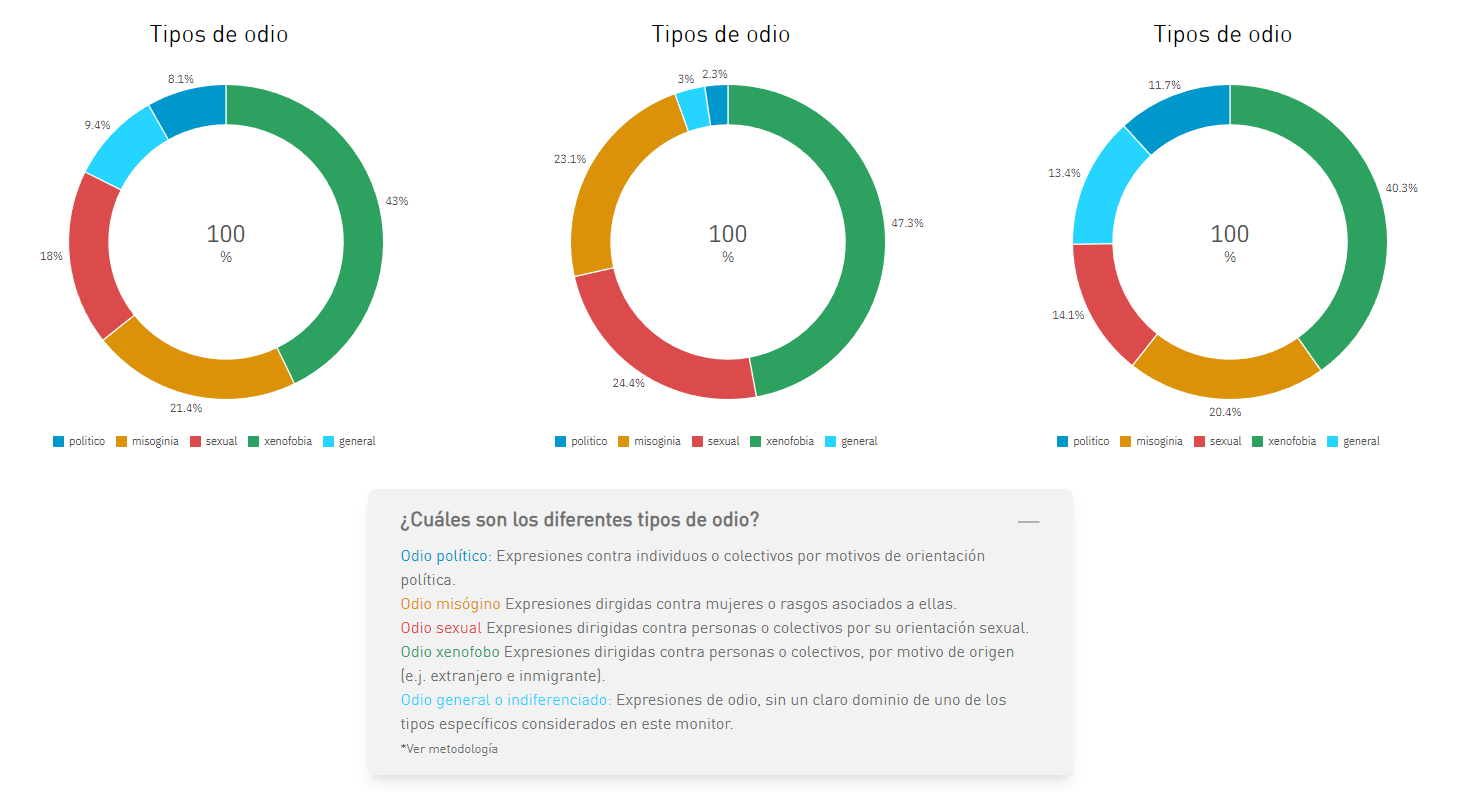
\includegraphics[scale=0.25]{Plantilla_TFG_ingles_2019/imagenes/hatemedia2.png}}
\end{figure}


